\documentclass[a4paper,kulak]{kulakarticle}

\usepackage[dutch]{babel}
\usepackage{hyperref}
\usepackage{graphicx}
\usepackage{amsmath, amssymb, amsthm}
\usepackage{siunitx}
\usepackage[toc,page]{appendix}
\renewcommand\appendixname{Bijlage}
\renewcommand\appendixpagename{Bijlagen}
\usepackage{pdfpages}


\title{Tussentijds verslag}
\author{Groep 1}
\date{\today}

\begin{document}
		\maketitle
	
\section{Inleiding}

\subsection{Probleemstelling}
Meer en meer zien we een groei van het verstedelijkt gebied. De verstedelijking breidt zich uit en de groei wordt versterkt. Met deze groei nemen ook de problemen toe. Als we terugkijken in de tijd, zien we een meermaals voorkomende situatie. Steden zitten in een bloeiperiode, bereiken een verzadigingspunt en vallen dan ineen. Zo was er ook de val van Rome, nadat deze een hoogtepunt had bereikt. Oude steden hadden dan wel een kleiner bereik, maar de relatie tussen technologie en stedelijke groei blijft dezelfde.\cite{smartcities} We staan opnieuw voor een keerpunt, waarbij we moeten kiezen tussen groeien of blijven steken.

We moeten de technologie de we voor handen hebben kunnen gebruiken om dit vastlopen te voorkomen. Met andere woorden moeten we van onze steden 'slimme steden' maken. Iedereen krijgt te maken met deze veranderingen in het dagelijkse leven en zou dus moeten weten wat dit allemaal inhoudt. Daarom is het nodig mensen bewust te maken van het nut van deze slimme steden.

\subsection{Slimme steden}

Maar wat zijn slimme steden nu juist? Met slim wordt de technologische innovatie bedoeld die opweegt tegen fysieke beperkingen. Een stad is een gebied van interacties en bijgevolg ook problemen en confrontaties \cite{sc}. In een kleine ruimte worden verscheidene dingen geconcentreerd samengebracht. Een stad heeft een veelheid aan functies en is pas doelmatig \cite{synoniemen} wanneer ze hierin slaagt. Een slimme stad wordt bereikt door stedelijke werking efficiënt te laten verlopen en het vereenvoudigen van (openbare) diensten. Informatie- en communicatietechnologie, beter gekend als ICT, wordt gecombineerd met dagdagelijkse objecten om die interacties te verbeteren en stedelijke problemen te verminderen. Dit idee is voorlopig nog steeds een utopie, maar werkt als een drijfveer \cite{proconsc}.

\subsection{Zelfrijdende auto's}

Een van de middelen om de efficiëntie te verhogen in een stad is door het invoeren van zelfrijdende auto's die zelfstandig kunnen deelnemen aan het verkeer. Niet alleen kan de bestuurder zijn tijd gebruiken voor andere zaken, maar ook files worden verminderd. De auto's kunnen dichter op elkaar volgen en het naleven van de verkeersregels is verzekerd. Dit zorgt ook voor een vermindering van verkeersongevallen. Het concept heeft niet alleen maar voordelen, zo zouden hackers kunnen zorgen voor enorme verkeersproblemen. Ook een grote inkomst van de overheid valt weg wanneer geen verkeersboetes of accijnzen op brandstof worden betaald. Daardoor zullen er meer belastingen op elektriciteit moeten geheven worden. Daarnaast zullen verschillende beroepen zoals buschauffeurs, rijinstructeurs en vrachtwagenchauffeurs overbodig worden, wat voor meer werkeloosheid onder minder geschoolden zal leiden\cite{procontracars}.

Ondanks de overheid autonoom rijden stimuleert, staat men in België sceptisch tegenover het idee, toch is er sprake van een grote marktpotentie. Bij de nieuwste auto's is er al sprake van een zeker mate van zelfstandigheid, zo kan men gealarmeerd worden bij het naderen van een andere bestuurder.Bekende bedrijven zoals Google, Apple en Uber zijn volop bezig met de ontwikkeling van deze autonome wagens. Google werkt samen met verschillende autobouwers, waaronder Audi en Toyota en Apple heeft met hun project 'Titan' al meer dan 50 autonome wagens op de openbare weg rijden \cite{bedrijven}. Er is geen ontkennen aan, zelfrijdende auto's hebben een toekomst.

\section{Ontwerp}
De zelfrijdende miniatuur robotwagen moest zich volgens een voorgeprogrammeerde route door een modelstad kunnen voortbewegen waarbij de modelstad bestaat uit negen identieke kruispunten. Hierbij volgt de miniatuur robotwagen een volglijn. Bij de kruispunten hangen er stoplichten op 75mm hoogte, en de miniatuur robotwagen moet kunnen detecteren wanneer hij al dan niet mag door rijden. Ook moet de miniatuur robotwagen een voorligger/obstakel kunnen detecteren en stoppen om een botsing te vermijden indien nodig. De afmetingen van de miniatuur robotwagen worden ook beperkt door de weg tot 300mm hoog en 250mm breed. De lengte van het voertuig valt vrij te kiezen maar moet dus wel haalbaar zijn. 
\subsection{Chassis}
Nadat we de ruwe richtlijnen wisten begon het ontwerpproces bij het uitkiezen van de te gebruiken onderdelen en het afwegen van de voordelen en nadelen van bepaalde onderdelen. Er bestaan ontzettend veel verschillende apparatuur om zo’n miniatuur voertuigje te maken, en normaal gezien zouden er dus ontzettend veel keuzes gemaakt moeten worden tussen de verschillende componenten. Voor deze opdracht werden onze keuzes echter gelimiteerd tot de componenten die beschikbaar waren op een materiaallijst. Er waren dus maar een paar verschillende belangrijke keuzes die moesten gemaakt worden, de motor, sensoren analoog/digitaal, het breadboard, de wielen, de microcontroller, het chassis en de soort batterij. Voor de wielen van ons voertuig hebben we gekozen voor de kleinste wielen met diameter 32mm. We hebben voor deze wielen gekozen omdat ze meer nauwkeurigheid bieden bij het roteren van het voertuig, en minder kracht nodig hebben om rond gedraaid te worden. Het nadeel aan deze wielen is echter wel dat de topsnelheid lager ligt. De motor die we het meest compatibel vonden met deze wielen was de 30:1 HP. Deze motor gaf ons nog de hoogste topsnelheid met de wielen die we gekozen hadden. Om dit te bepalen hebben we enkele berekeningen uitgevoerd met hoeveel toeren per minuut de motor maximaal kan draaien en de omtrek van de wielen. Deze wielen en motoren zullen we plaatsen aan de voorkant van onze wagen. De motoren worden aan de onderkant van het chassis bevestigd om zo ons chassis hoger van de grond te krijgen. Zo past de lijnsensor er ook nog onder. Deze komen aan de voorkant zodat het sturen van de wagen vergemakkelijkt . De balcaster zullen we in het midden vanachteren plaatsen. Deze zullen we proberen op dezelfde hoogte te plaatsen als de wielen door er plastic verhoog plaatjes eronder te bevestigen. Hierdoor zal het chassis een minimale hoek maken met de grond waardoor de sensoren gerichter zullen staan. De Rasberry Pi plaatsen we op vier afstandsbussen van 15mm hoog waardoor hij op een verhoogje komt te staan. Dit doen we om wat meer ruimte te creëren voor de sensoren, motoren, wielen en Maker Beams die nog op het chassis moeten komen.Op de Rasberry komen 2  breadboard tiny’s die aan elkaar gelinkt zijn. Achter de Rasberry Pi ter hoogte van onze balcaster zullen we de powerbank op het chassis plaatsen. Deze past jammer genoeg juist niet onder de Rasberry waardoor hij niet onder het verhoogje kan. De powerbank zorgt met zijn gewicht ervoor dat het massamiddelpunt meer naar achteren en omlaag komt te liggen wat zorgt voor extra stabiliteit. De powerbank is ook gemakkelijker aan te sluiten op de Rasberry Pi en levert het juiste voltage voor de Rasberry Pi om te functioneren.
\subsection{Sensoren}
De kleurensensor zullen we bevestigen aan een makerbeam op een hoogte van 75mm van de grond zodat deze het verkeerslicht op dezelfde hoogte kan detecteren. Hierbij zullen we een constructie van makerbeams maken die ervoor kan zorgen dat we de kleurensensor kunnen verplaatsen in alle richtingen indien nodig. Deze constructie bestaat uit een makerbeam die horizontaal in het midden van ons chassis ligt onder de Rasberry Pi met daar op een makerbeam verticaal omhoog aan het rechter uiteinde.. Hierop bevestigen we een horizontale makerbeam met de kleurensensor. 
Voor de afstand sensor hebben we gekozen voor een analoge sensor, zodat we onderscheid kunnen maken hoe ver een voorligger ligt. Doordat we dit onderscheid kunnen maken moet onze miniatuur robotwagen niet direct stoppen als hij een voorligger detecteert, maar kunnen we zorgen dat hij eerst wat trager rijdt en dan volledig stopt. Deze afstand sensor plaatsen we logischer wijze aan de voorkant van ons chassis aan een makerbeam zodat hij zo vroeg mogelijk een voorligger kan detecteren aangezien zijn detectie bereik maar 100mm is. 
De reflectiesensor wordt gebruikt om de volglijn te detecteren. Hierbij hebben we een digitale sensor gekozen omdat deze compatibel is met de Rasberry Pi microcontroller en de sensor geen onderscheid moet kunnen maken tussen de soort lijn. Deze wordt aan de voorkant onder het chassis bevestigd met behulp van afstandsbuizen zodat deze de volglijn als eerst detecteert en we zo sneller correcties kunnen uitvoeren. Aangezien de sensor ook dicht bij de wielen ligt zal het wagentje ook nauwkeuriger bewegen.
\section{Evaluatie}

\subsection{Planning}

Tot en met week 5 is alles verlopen zoals gepland en vastgelegd in de Gantt-grafiek. De documenten met betrekking tot de planning zijn afgewerkt net zoals het ontwerp van de chassis en het CAD-model. Het team was van plan om te beginnen met de assemblage in week 6, echter wordt dit een week uitgesteld vanwege een probleem met de microcontroller. Het programmeren van de sensoren verliep vlot, enkel het programmeren in verband met de aansturing van het wagentje zal iets meer tijd innemen dan ingerekend. Dit wordt dan wel gecompenseerd met het CAD-model die minder tijd innam dan voorspeld, waardoor we nog altijd op schema zitten. Ook het schrijven van het verslag verloopt volgens schema. De tijd voorzien tijdens de lessen wordt efficiënt gebruikt, waardoor het werk buiten de lessen wordt beperkt tot een minimum \cite{opgave}.

\subsection{Financiën}

Doordat we de laatste keuze hadden bij het bestellen, liepen we achter op onze planning, onze financiële situatie kende hier dan weer voordelen door. We zijn gestart met een budget van 3500 kredietpunten, dat werd gereduceerd tot een tegoed van 1768 na het plaatsen van een eerste bestelling. In deze  order \cite{woordenlijst} werden alle grote onderdelen en zaken die we zeker nodig hadden besteld.  Aan onze eerste levering ontbraken nog Makerbeams en afstandsbussen. Onze tweede bestelling zou 61 kredietpunten kosten, waardoor we stranden op een budget van 1646 credits. Door eigen keuze wordt het chassis zelf ontworpen en 3D-geprint. Dit is vermoedelijk een grote kost die werd geschat op 500 kredietpunten. Onze financiële toestand zorgt ervoor dat we in een comfortabele situatie zitten. We kunnen het ons veroorloven om fouten te maken en risico's te nemen. 



	\bibliographystyle{plain} %De stijl van de bibliografie
	\bibliography{bibliografietv} %De bibliografie zelf
\begin{appendices}
	\section*{Planningsdocumenten} %De goede titel
	\renewcommand\refname{} %De oude titel verwijderen
	\vspace{-2\bigskipamount} %De cursor terugzetten
	\bibliographystyle{plain} %De stijl van de bibliografie
%	\bibliography{bibliografietv} %De bibliografie zelf

	
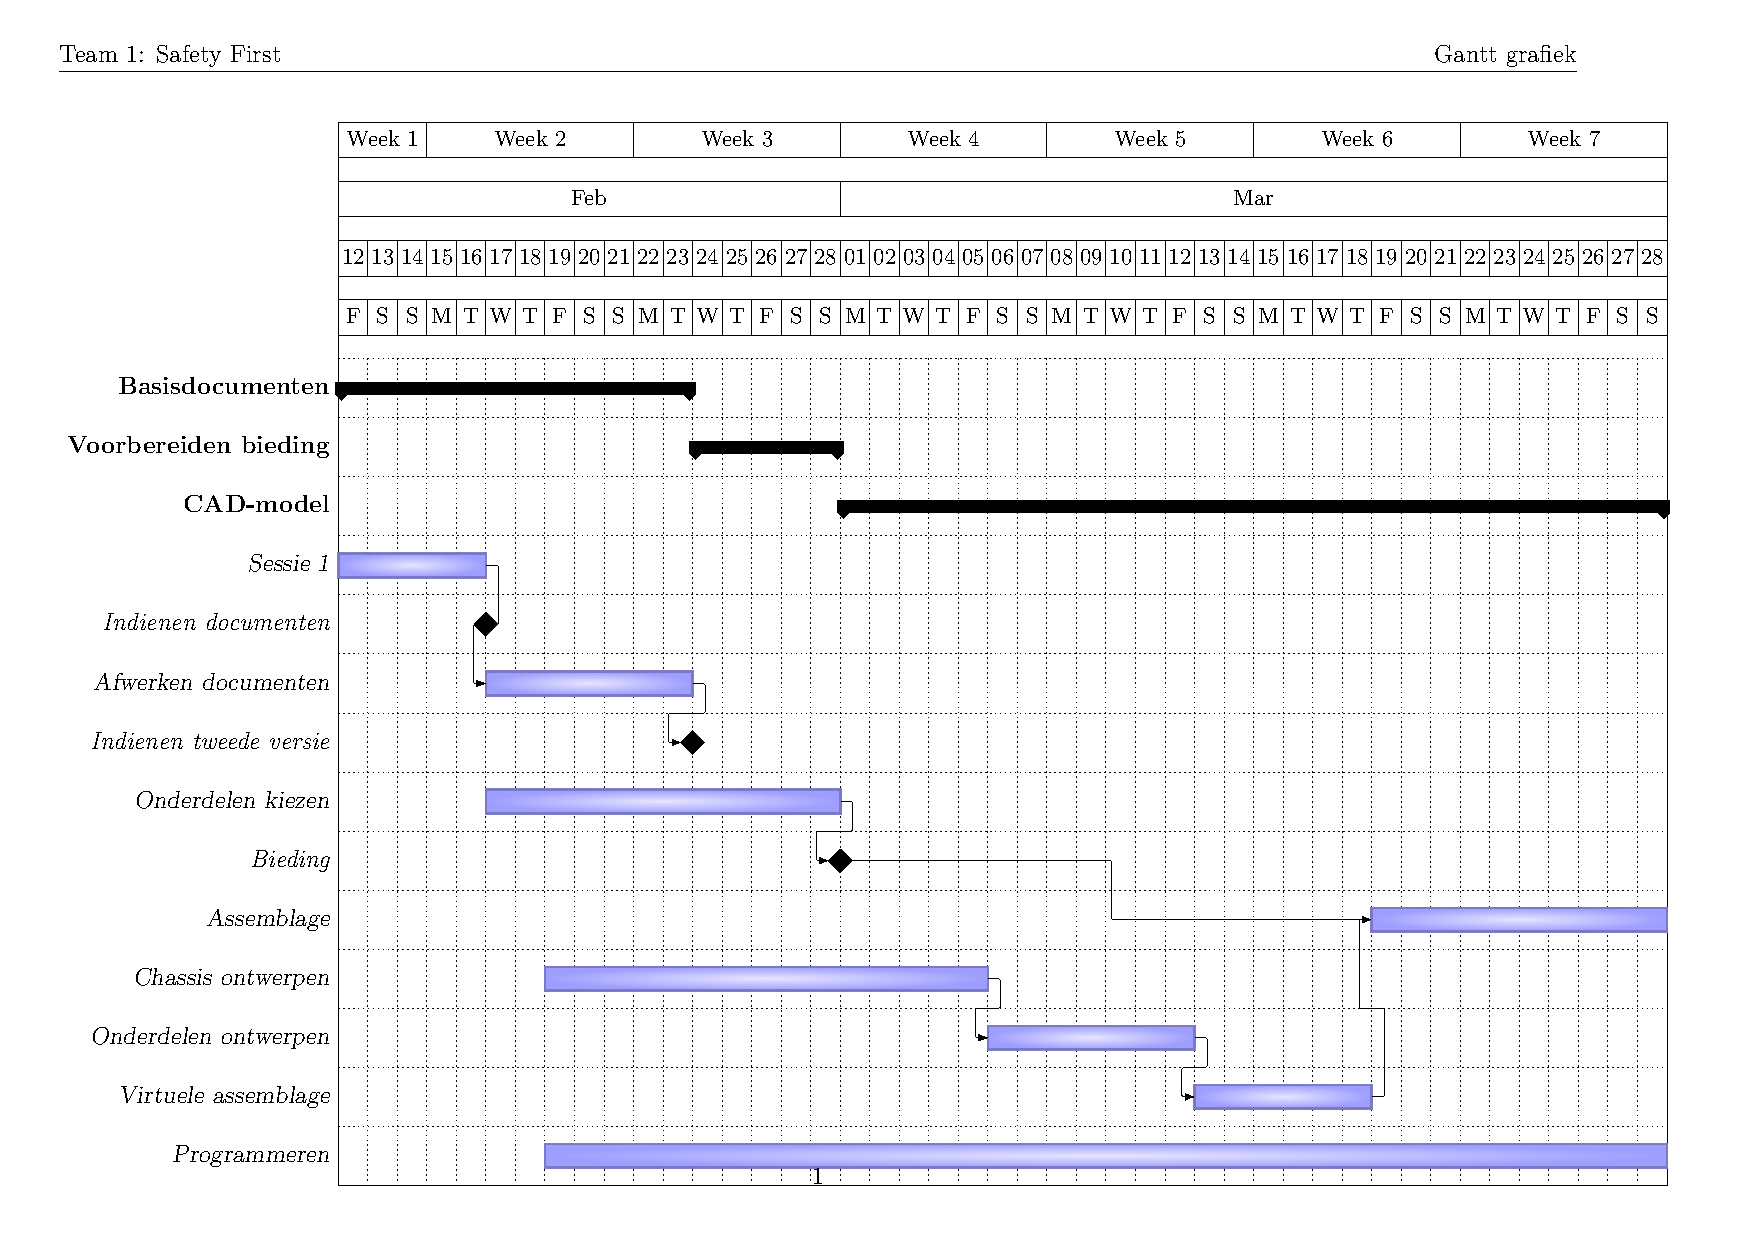
\includepdf[pages=-]{ganttchart.pdf}

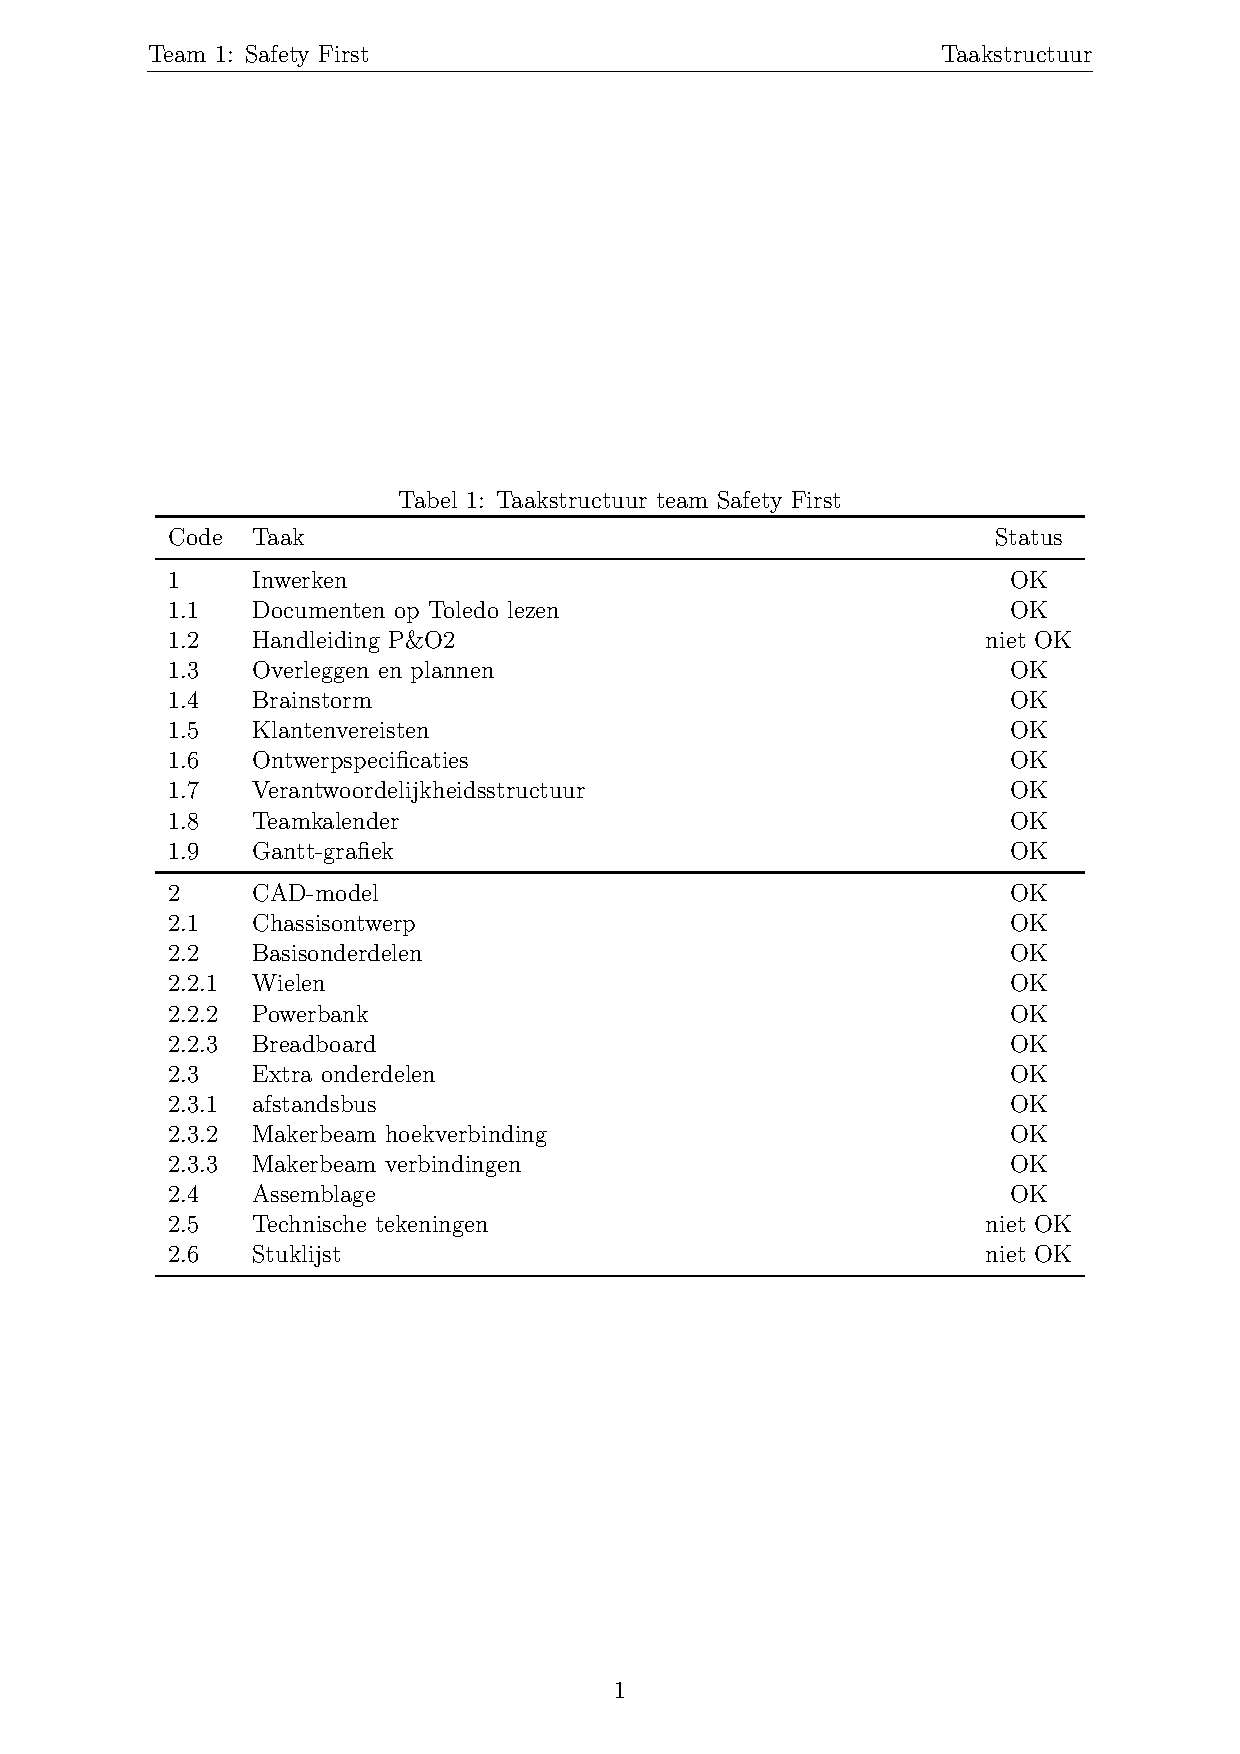
\includepdf[pages=-]{taakstructuur.pdf}

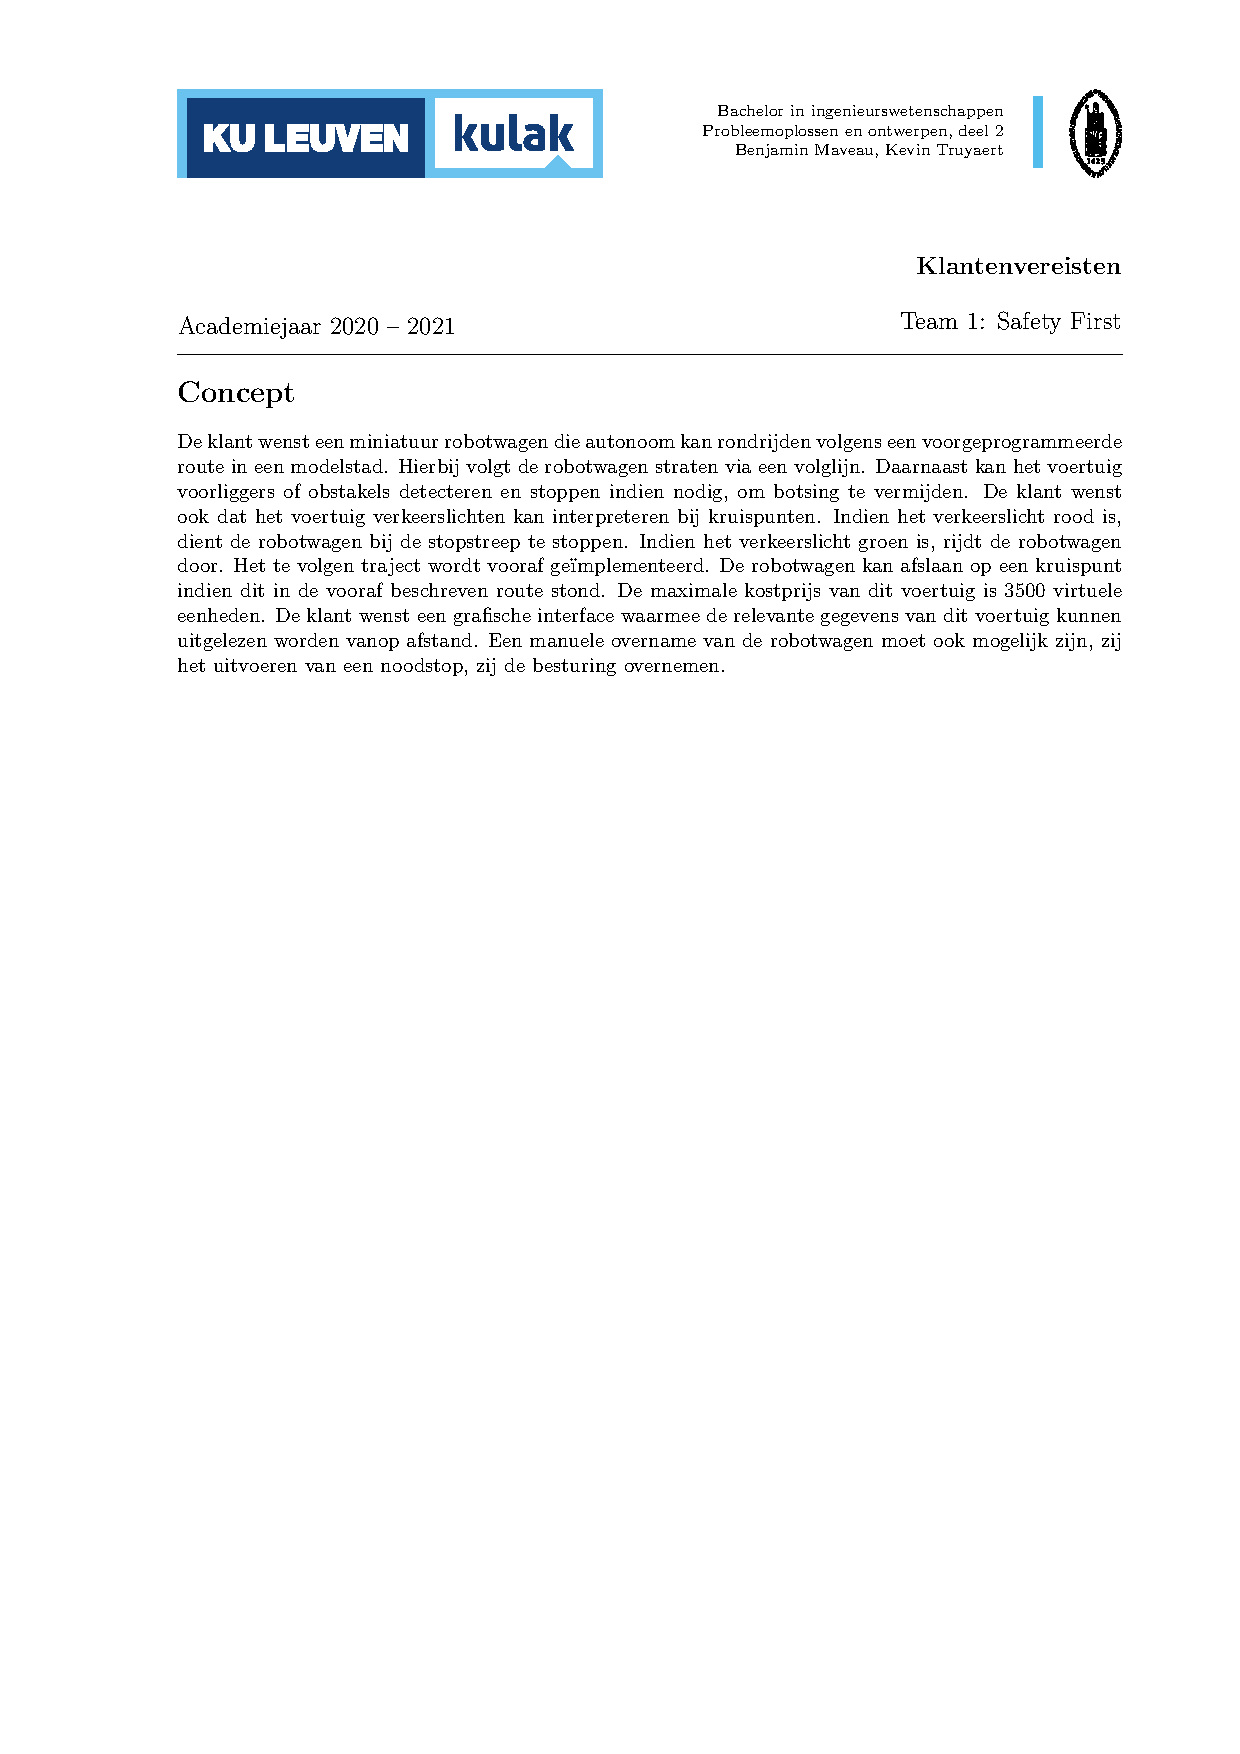
\includepdf[pages=-]{klantenvereisten.pdf}
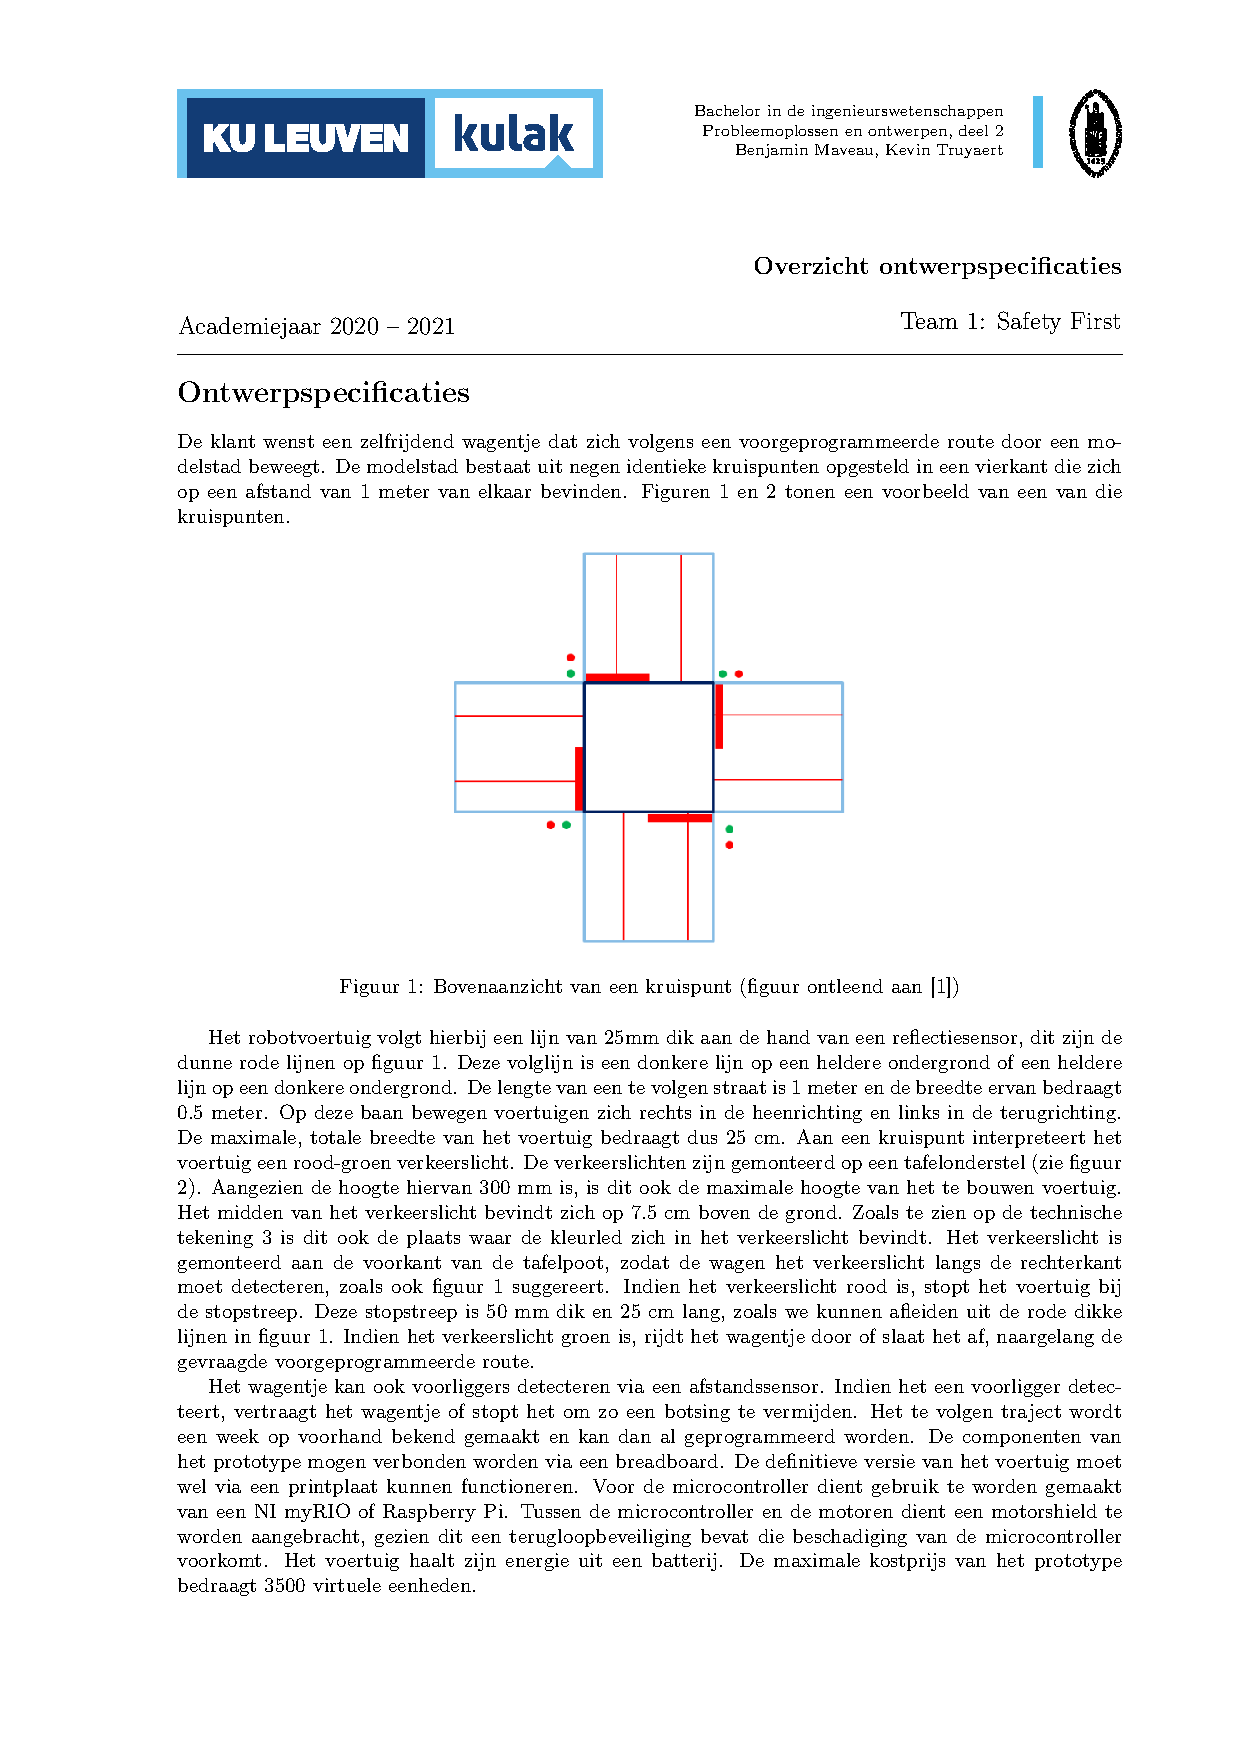
\includepdf[pages=-]{ontwerpspecificaties.pdf}

\end{appendices}




\end{document}